% ============================================================================
\section{Multimodality}
% ============================================================================

% --- Vision--Language Models (VLMs): Rohit Bandaru blog tour ---
\begin{frame}[t]{Vision--Language Models: why pair vision with language?}
  \begin{itemize}
    \item Strong \textbf{image embeddings} are useful, but many tasks still need a way to \textbf{say what you want} in words (``what species of bird is this?'', ``read the sign in the corner'').
    \item \textbf{Language} makes it easy to specify new tasks without collecting a fresh classification label set for every concept---a path to flexible, user-steerable vision AI.
    \item \textbf{Nomenclature (informal):} an \textbf{LLM} is language-first; a \textbf{VLM} adds a \textbf{vision encoder} so the stack can \textbf{condition on images}; an \textbf{MLLM} usually means several modalities (image, video, audio) in one family.
  \end{itemize}
  \vfill
  {\scriptsize Bandaru, \textit{Vision Language Models} (blog, Aug.\ 2025), \href{https://rohitbandaru.github.io/blog/Vision-Language-Models/}{rohitbandaru.github.io/blog/Vision-Language-Models/}.}
\end{frame}

\begin{frame}[t]{Fusion Patterns: Where do image tokens meet the LLM?}
  \begin{itemize}
    \item Early fusion: build one long token sequence (visual tokens + text tokens) and run attention over the mixture---what most ``native'' VLMs aim for today.
    \item Middle fusion: insert vision cross-attention inside some transformer blocks (common when adapting a legacy text-only stack such as early LLaMA~3.2).
    \item Late fusion: combine modalities only at the end---usually too weak for open-ended captioning/VQA because the LLM never gets rich visual state early enough.
    \item Images create many tokens; good designs compress visual length (pooling, grouping, tiling) before the LLM sees them.
  \end{itemize}
\end{frame}

\begin{frame}[t]{Early Fusion approaches: MLP Adapter}
  \begin{itemize}
    \item Freeze (or lightly train) a strong ViT; map its patch tokens through a small MLP projector into the LLM embedding width, then concatenate with text tokens.
    \item Simple, stable, and very common in open recipes (LLaVA, LLaMA~4-style early fusion, PaliGemma~2, DeepSeek-VL, \ldots).
  \end{itemize}
  \centering
  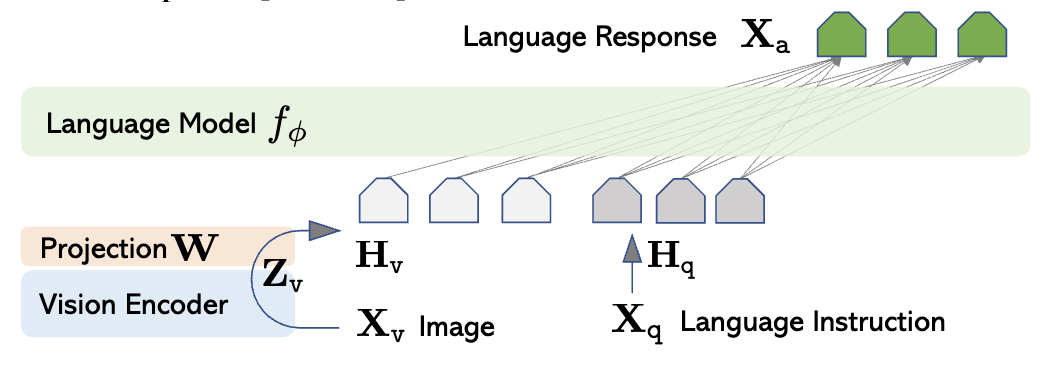
\includegraphics[width=\textwidth,height=0.58\textheight,keepaspectratio]{assets/New-Lecture-Transformers/bandaru_vlm_llava_architecture.png}
  \vspace{0.15em}
  {\scriptsize Diagram from Bandaru. Paper: Liu et al., LLaVA, \href{https://arxiv.org/abs/2304.08485}{arXiv:2304.08485}.}
\end{frame}

\begin{frame}[t]{Early Fusion approaches: Cross-Attention}
  \begin{itemize}
    \item A small \textbf{adapter} uses learned query vectors that \textbf{cross-attend} to ViT tokens and output a \textbf{fixed small} set of visual summaries for the LLM.
  \end{itemize}
  \centering
  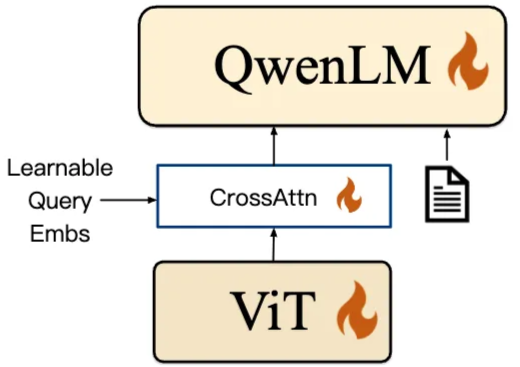
\includegraphics[width=\textwidth,height=0.58\textheight,keepaspectratio]{assets/New-Lecture-Transformers/bandaru_vlm_qwen_vl_adapter.png}
  \vfill
  {\scriptsize Diagram from Bandaru (Qwen-VL ``position-aware'' adapter).}
\end{frame}

% \begin{frame}[t]{Unified image \emph{tokens}: Chameleon-style early fusion}
%   \begin{itemize}
%     \item Some stacks \textbf{quantize} images to discrete codes (VQ-VAE), then treat them like extra \textbf{text-like tokens} inside one decoder.
%     \item Nice for \textbf{tight multimodal reasoning}; heavier data and training pipeline than ``ViT patches + adapter.''
%   \end{itemize}
%   \centering
%   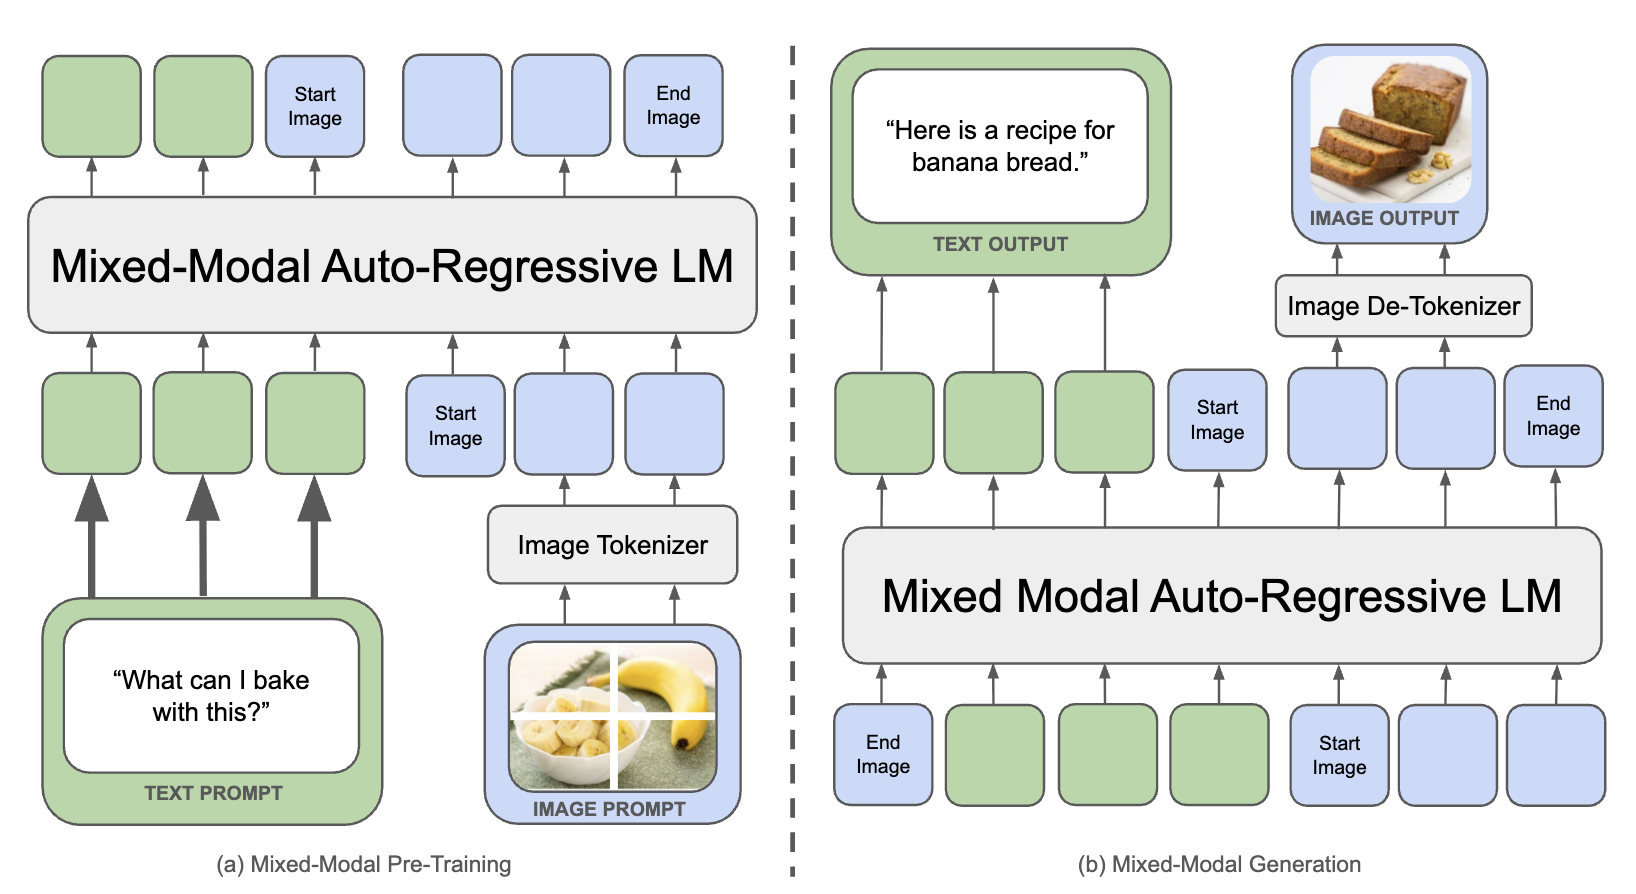
\includegraphics[width=\textwidth,height=0.55\textheight,keepaspectratio]{assets/New-Lecture-Transformers/bandaru_vlm_chameleon_architecture.png}
%   \vspace{0.15em}
%   {\scriptsize Diagram from Bandaru. Paper: Meta Chameleon, \href{https://arxiv.org/abs/2405.09818}{arXiv:2405.09818}.}
% \end{frame}

\begin{frame}[t]{Middle Fusion Approaches: Flamingo}
  \begin{itemize}
    \item Keep a pretrained ViT and LLM frozen; insert Perceiver resamplers (compress variable tokens $\to$ fixed count) and gated cross-attention blocks inside the LLM stack.
  \end{itemize}
  \centering
  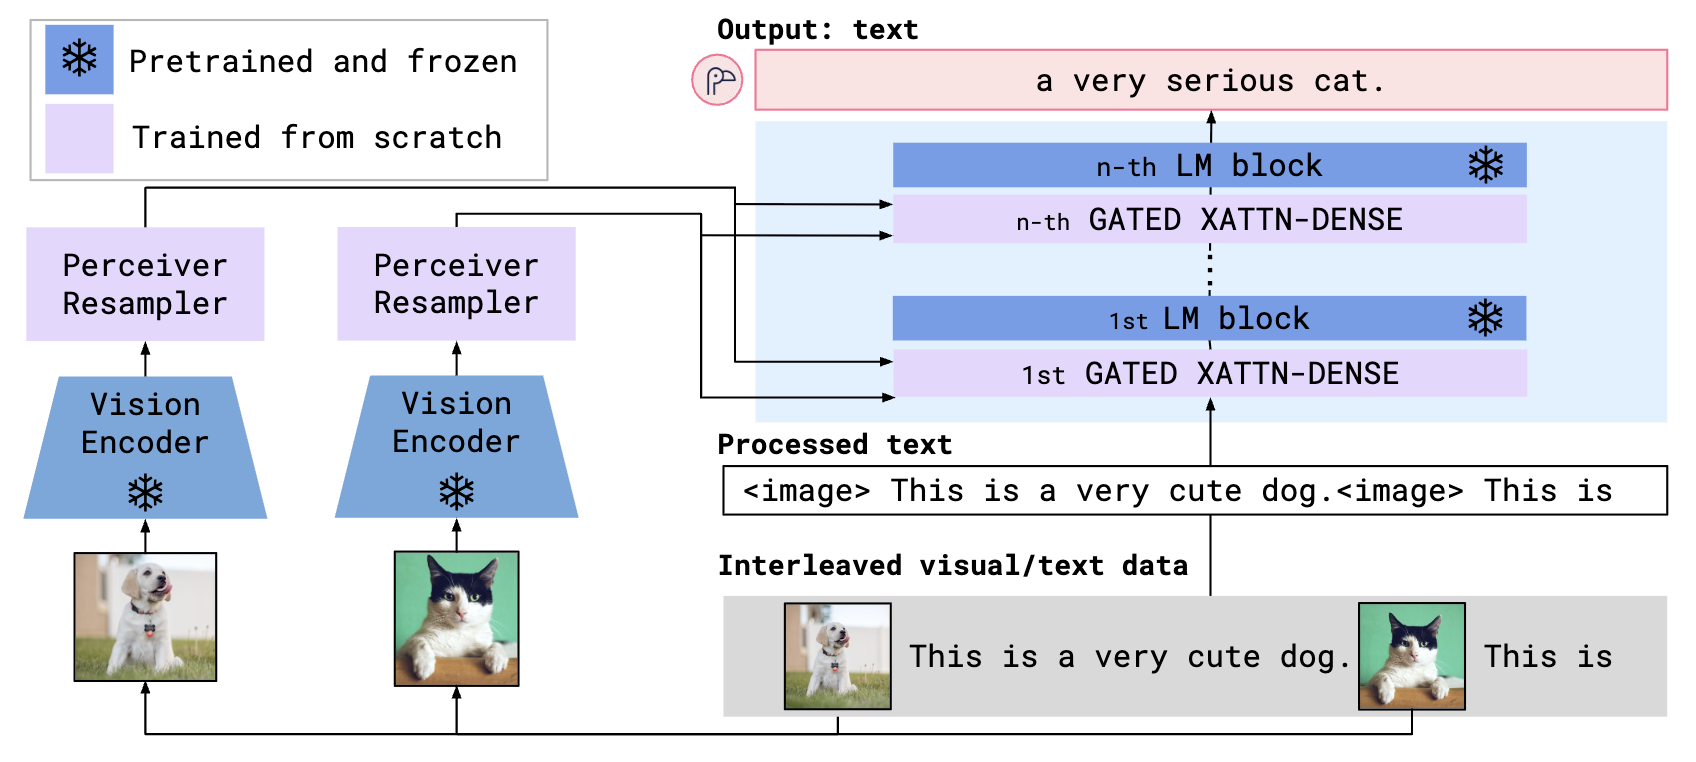
\includegraphics[width=\textwidth,height=0.52\textheight,keepaspectratio]{assets/New-Lecture-Transformers/bandaru_vlm_flamingo_architecture.png}
  \vfill
  {\scriptsize Diagram from Bandaru. Paper: Alayrac et al., Flamingo, \href{https://arxiv.org/abs/2204.14198}{arXiv:2204.14198}.}
\end{frame}

\begin{frame}[t]{Mid Fusion Approaches: LLaMA 3}
  \begin{itemize}
    \item \textbf{ViT encoder:} 32-layer ViT trained CLIP-style for image-text alignment; features extracted from multiple layers.
    \item \textbf{Decoder:} Image cross attention in every fourth block (no gating on cross attention).
    \item \textbf{Mid fusion} suits LLaMA 3's text-first design; LLaMA 4 moves to early fusion (MLP adapter) for true multimodal training.
  \end{itemize}
\end{frame}


% \begin{frame}[t]{Training in stages (example: BLIP-2)}
%   \begin{itemize}
%     \item Stage~1 trains a \textbf{Q-Former} adapter with several objectives (contrastive, matching, captioning) while LLM weights stay \textbf{frozen}.
%     \item Stage~2 \textbf{concatenates} Q-Former outputs to the LLM inputs and finetunes for generation---a template many recipes echo (alignment $\to$ instruction).
%   \end{itemize}
%   \centering
%   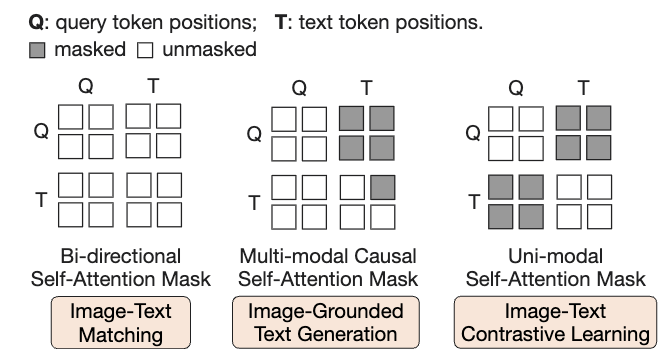
\includegraphics[width=\textwidth,height=0.52\textheight,keepaspectratio]{assets/New-Lecture-Transformers/bandaru_vlm_blip2_training_stages.png}
%   \vspace{0.15em}
%   {\scriptsize Diagram from Bandaru. Paper: Li et al., BLIP-2, \href{https://arxiv.org/abs/2301.12597}{arXiv:2301.12597}.}
% \end{frame}

% \begin{frame}[t]{Scaling training (example: Qwen-VL pipeline)}
%   \begin{itemize}
%     \item Large open recipes often: \textbf{massive image--text pretrain} $\to$ multitask midtrain $\to$ short, high-quality \textbf{instruction} finetuning (sometimes freezing ViT at the end).
%     \item Later variants add \textbf{video}, \textbf{dynamic resolution}, and \textbf{long-context} stages---each step uses fewer examples but higher signal.
%   \end{itemize}
%   \centering
%   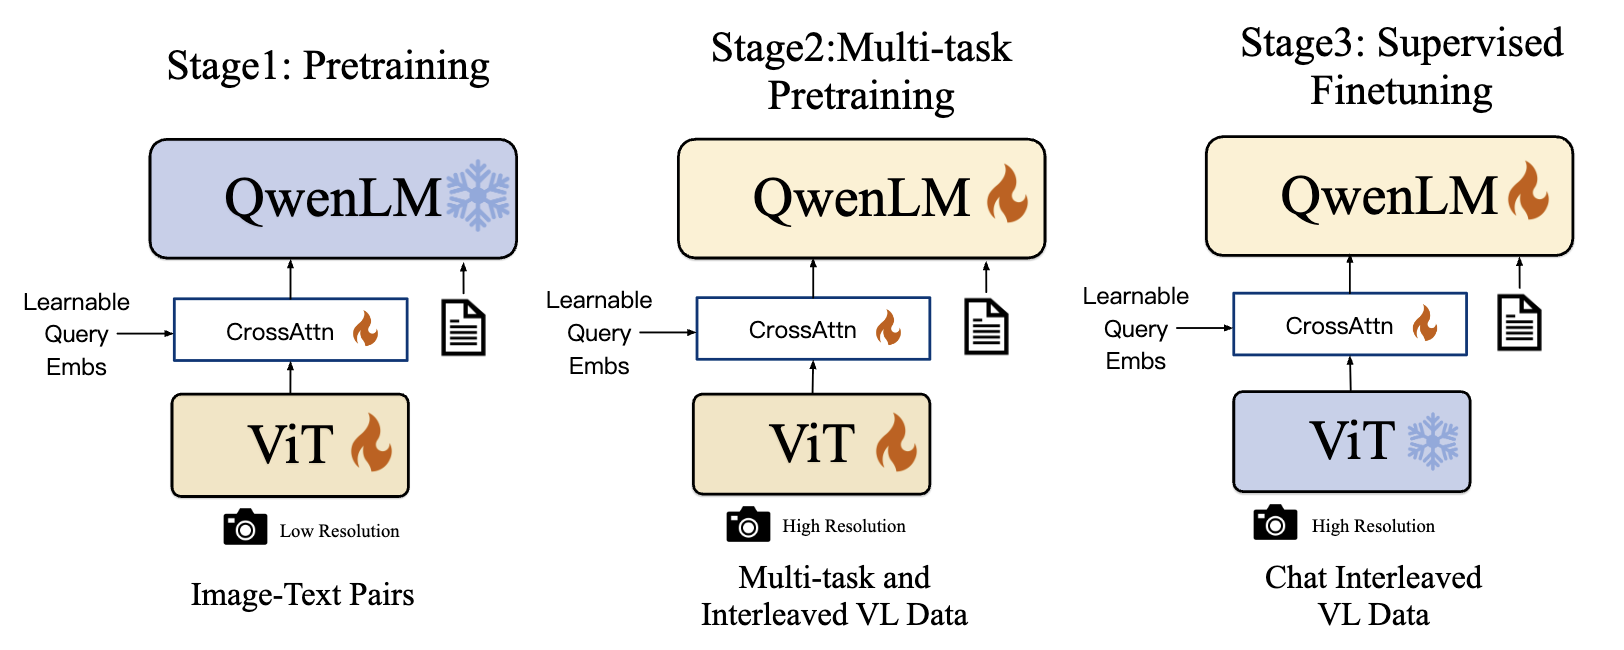
\includegraphics[width=\textwidth,height=0.48\textheight,keepaspectratio]{assets/New-Lecture-Transformers/bandaru_vlm_qwen_vl_training_stages.png}
%   \vspace{0.15em}
%   {\scriptsize Diagram from Bandaru (Qwen-VL training stages).}
% \end{frame}

% \begin{frame}[t]{Video: token counts explode (and why compression matters)}
%   \begin{itemize}
%     \item Naively tokenizing \textbf{every frame} at full FPS produces enormous context (cost scales like attention length).
%     \item Practical systems \textbf{subsample in time}, use \textbf{3D patch} encoders to merge frames, or learn \textbf{content-aware} compressors (example below: run-length style redundancy).
%   \end{itemize}
%   \centering
%   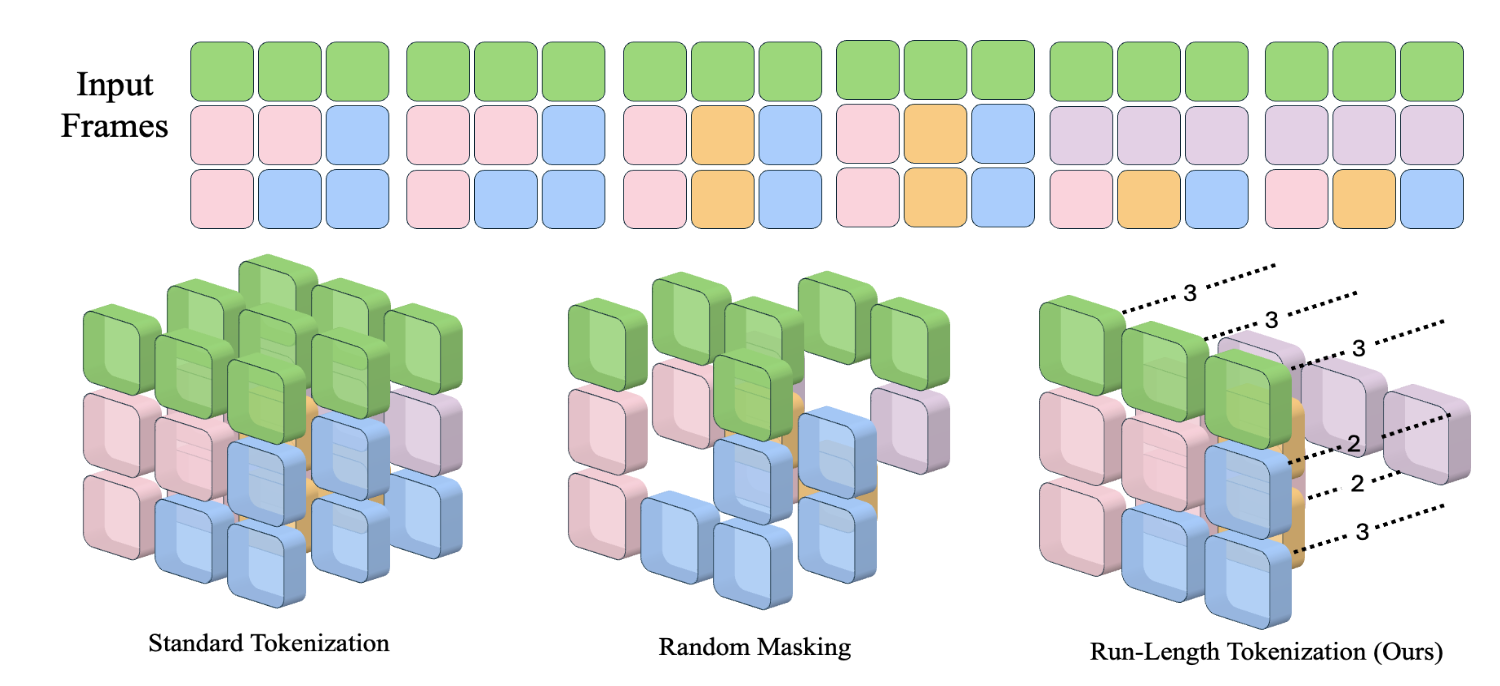
\includegraphics[width=\textwidth,height=0.48\textheight,keepaspectratio]{assets/New-Lecture-Transformers/bandaru_vlm_rlt_video_compression.png}
%   \vspace{0.15em}
%   {\scriptsize Diagram from Bandaru (Run-Length Tokenization sketch). Paper: Choudhury et al., \href{https://arxiv.org/abs/2411.05222}{arXiv:2411.05222}.}
% \end{frame}

% \begin{frame}[t]{Instruction-tuned VLM (LLaVA paper figure)}
%   \centering
%   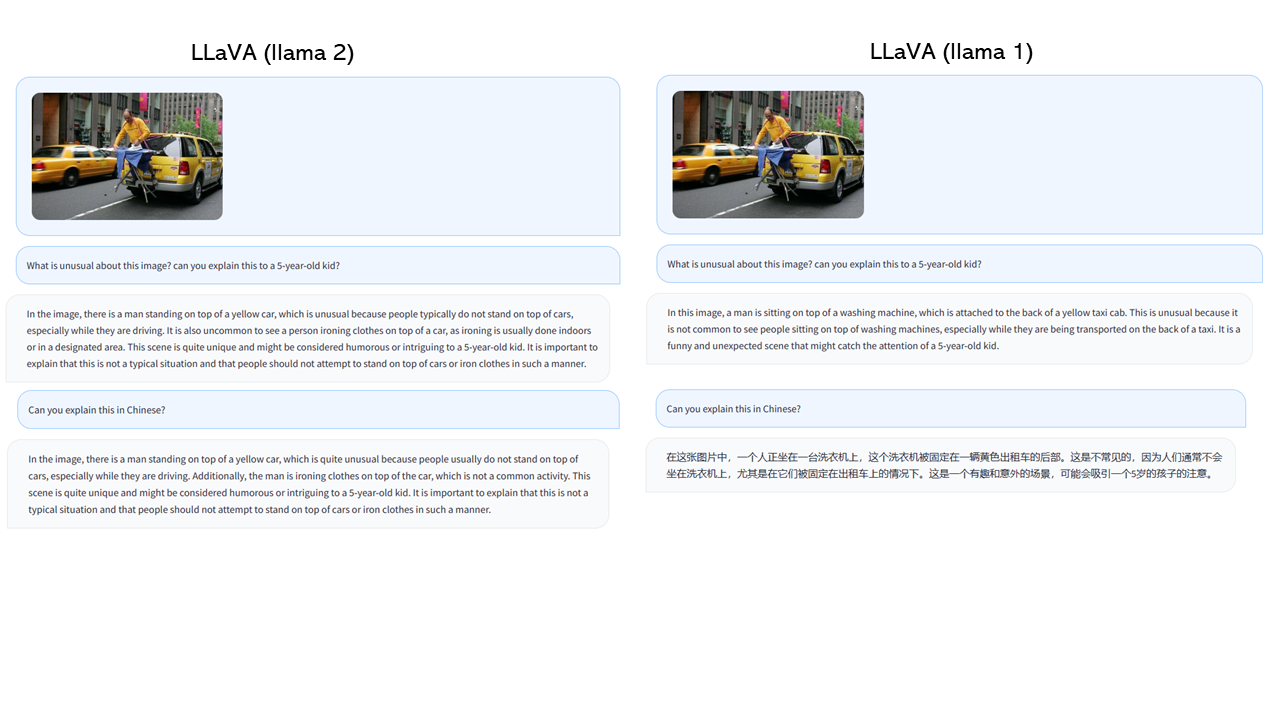
\includegraphics[width=\textwidth,height=0.72\textheight,keepaspectratio]{assets/New-Lecture-Transformers/llava_vlm_example.png}
%   \vfill
%   {\scriptsize Liu et al., ``Visual Instruction Tuning'' (LLaVA), \href{https://arxiv.org/abs/2304.08485}{arXiv:2304.08485}.}
% \end{frame}

